\documentclass{article}
  \usepackage{amsmath}
  \usepackage{amssymb}
  \usepackage{graphicx}
  \usepackage{float}
  \usepackage{setspace}
  \usepackage{stata}
  \usepackage{bm}
  \usepackage{amssymb}
  \usepackage{listings}
\topmargin=-1.2cm \oddsidemargin=0.1cm \evensidemargin=0.1cm
\textwidth=16 true cm \textheight=23 true cm

\font\euler=EUSM10 \font\eulers=EUSM7

\begin{document}
\title{Advanced Microeconomics\\Assignment $3^{\text{rd}}$}
\author{{\normalsize SHENG Hao, 1401211818, via \LaTeX}}
\date{\today}

\maketitle

\def \Pr{{\rm Pr}}
\baselineskip 0.6cm
\section*{Q1}
\subsection*{1)}
Notice that $f(x_1,x_2)$ can be written as $g(h(x_1,x_2))$ where $g(\cdot)$ is strictly increasing function and $h(\cdot)$is homogeneous of degree one, i.e.
\begin{equation}
	h(tx_1,tx_2) = t^kh(x_1,x_2),\quad \forall t>0, \quad k=1
\end{equation}
So, $f(x_1,x_2) = f(x^{'}_1,x^{'}_2)$ is to say $h(x_1,x_2) = h(x^{'}_1,x^{'}_2)$. Thus,
\begin{equation}
	f(\alpha x_1, \alpha x_2) = f(\alpha^k h(x_1,x_2))=f(\alpha^k h(x_1,x_2)) = f(\alpha x^{*}_1, \alpha x^{*}_2)
\end{equation}
\rightline{$\blacksquare$}

\subsection*{2)}
\begin{align}\notag
	\text{MRTS}_{\alpha x_1,\alpha x_2} &= \frac{\frac{\partial f(\alpha x_1, \alpha x_2)}{\partial x_1}}{\frac{\partial f(\alpha x_2, \alpha x_2)}{\partial x_2}}
	= \frac{g^{'}(h(\alpha x_1, \alpha x_2))\frac{\partial h(\alpha x_1, \alpha x_2)}{\partial x_1}}{g^{'}(h(\alpha x_1, \alpha x_2))\frac{\partial h(\alpha x_1, \alpha x_2)}{\partial x_2}} 
	= \frac{\alpha^{k-1} \frac{\partial h(x_1, x_2)}{\partial x_1}}{\alpha^{k-1} \frac{\partial h(x_1, x_2)}{\partial x_2}}\\ \notag
	&=\frac{g^{'}(h( x_1,  x_2))\frac{\partial h( x_1,  x_2)}{\partial x_1}}{g^{'}(h( x_1,  x_2))\frac{\partial h( x_1,  x_2)}{\partial x_2}}
	= \frac{\frac{\partial h( x_1,  x_2)}{\partial x_1}}{\frac{\partial h( x_2,  x_2)}{\partial x_2}} \\ \notag
	&= \text{MRTS}_{ x_1, x_2} 
\end{align}
\rightline{$\blacksquare$}

\section*{Q2}
\subsection*{1)}
Profit maximization problem:
\begin{align}
	\notag \underset{x_1,x_2}{Max}\quad px_1^{a_1}x_2^{a_2}-w_1 x_1 - w_2 x_2
\end{align}
F.O.C gives us:
\begin{equation}
	\begin{cases}
	a_1 p x_1^{a_1-1} x_2^{a_2} &= w_1 \\ 
	a_2 p x_1^{a_1} x_2^{a_2-1} &= w_2
\end{cases}
\end{equation}
Solving it leads to the factor demand functions:
\begin{equation} \label{eq:FactorDemandFunction}
	\begin{cases}
		x_1 = (\frac{w_1}{a_1} (\frac{a_1}{a_2})^{a_2} (\frac{w_2}{w_1})^{a_1})^{\frac{1}{a_1 + a_2 -1}} \\
		x_2 = (\frac{w_2}{a_2} (\frac{a_2}{a_1})^{a_1} (\frac{w_1}{w_2})^{a_2})^{\frac{1}{a_1 + a_2 -1}}
	\end{cases}
\end{equation}
Substitute eq(\ref{eq:FactorDemandFunction})) into the $f(x_1,x_2)$, and solve $Q$:
\begin{align} \notag \label{eq:Supply1}
Q &= x^{a_1}_1 x^{a_2}_1\\
  &= (\frac{1}{p^{a_1+a_2}} (\frac{w_1}{a_1})^{a_1} (\frac{w_2}{a_2})^{a_2} )^{\frac{1}{a_1 + a_2 - 1}}
\end{align}

\subsection*{2)}
Cost minimization problem:
\begin{align}
\notag \underset{x_1,x_2}{Min}\quad w_1 x_1 + w_2 x_2 \\
\notag s.t.\quad f(x_1,x_2) = x_1^{a_1}x_2^{a_2} = Q
\end{align}
First order condition:
\begin{equation}
	\begin{cases}
	a_1 x_1^{a_1-1} x_2^{a_2} &= \lambda w_1 \\ 
	a_2 x_1^{a_1} x_2^{a_2-1} &= \lambda w_2		
	\end{cases}
\end{equation}
, where $\lambda$ is the undetermined coefficient.\\
And it's easy to check the S.O.C is satisfied. Solving it leads to the conditional factor demand functions:
\begin{equation}
	\begin{cases}
		x_1 = (Q (\frac{a_1}{a_2})^{a_2} (\frac{w_2}{w_1})^{a_1})^{\frac{1}{a_1 + a_2}} \\
		x_2 = (Q (\frac{a_2}{a_1})^{a_1} (\frac{w_1}{w_2})^{a_2})^{\frac{1}{a_1 + a_2}}		
	\end{cases}
\end{equation}
Such $x_1, x_2$ will determine the cost function as:
\begin{equation}
	C(Q,\bm{w}) = (Q w^{a_1}_1 w^{a_2}_2)^{\frac{1}{a_1 + a_2}} (\frac{a_1+a_2}{a_1}) (\frac{a_1}{a_2})^{\frac{a_2}{a_1+a_2}}
\end{equation}
Next, we look into the profit maximization problem based on cost function:
\begin{equation}
	\notag \underset{Q}{Max}\quad PQ-C(Q,\bm{w})
\end{equation}
Its first order condition:
\begin{equation}
	P = (w^{a_1}_1 w^{a_2}_2)^{\frac{1}{a_1+a_2}} Q^{\frac{1 - a_1 - a_2}{a_1 + a_2}} a^{\frac{-a_1}{a_1+a_2}}_1 a^{\frac{a_2}{a_1+a_2}}_2
\end{equation}
Solve $Q$ from the above,
\begin{equation}
	Q = (\frac{1}{p^{a_1+a_2}} (\frac{w_1}{a_1})^{a_1} (\frac{w_2}{a_2})^{a_2} )^{\frac{1}{a_1 + a_2 - 1}}
\end{equation}
, which is the same supply function as from first approach (see eq.(\ref{eq:Supply1}))
\section*{Q3}
As is defined in class,
\begin{equation}
	e(\bm{x}) = \left.\frac{\partial f(\alpha \bm{x})}{\partial {\alpha}} \frac{\alpha}{f(\alpha \bm{x})}\right|_{\alpha=1}
\end{equation}
Thus,
\begin{align} \notag
	e(\bm{x}) &= \frac{1}{f(\bm{x})} \sum _{i=1}^{n}(f_{x_i}(\alpha \bm{x})\frac{\partial{(\alpha_i x_i)}}{\partial \alpha_i})\\ \notag
	& = \sum _ {i=1}^{n} (\frac{\partial f(\bm{x})}{\partial x_i}\frac{x_i}{f(\bm{x})}) \\
	& = \sum _{i=1}^{n} E_i(\bm{x})
\end{align}
\rightline{$\blacksquare$}
\section*{Q4}
\subsection*{1)}
\begin{figure}[!h]
\centering
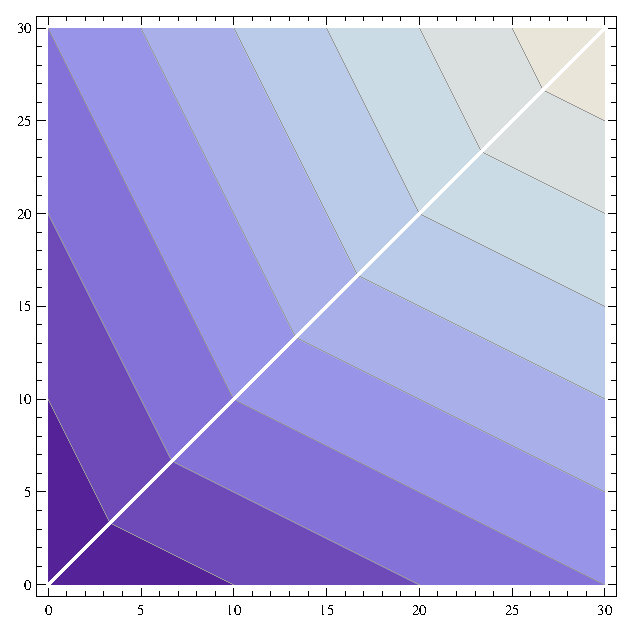
\includegraphics[width=0.5\linewidth]{AMIE2014Fa3.eps}
\caption{Isoquant of Production Function}
\end{figure}
\subsection*{2)}
Let the price of factor $x_1, x_2$ as $w_1, w_2$ respectively. The cost minimization problem:
\begin{align}
\notag \underset{x_1,x_2}{Min} \quad w_1 x_1 + w_2 x_2\\ 
\notag s.t.\quad f(x_1, x_2) = Q
\end{align}
Now we need to split in the following situation upon $\frac{w_1}{w_2}$
\begin{description}
\item[a) $\frac{w_1}{w_2}\in (0,\frac{1}{2})$] $\Rightarrow C(Q, \bm{w}) = w_1 Q$ and $\begin{cases}x_1=Q\\x_2=0\end{cases}$

\item[b) $\frac{w_1}{w_2} = \frac{1}{2}$] $\Rightarrow C(Q, \bm{w}) = w_1 Q = \frac{1}{2} w_2 Q$ and $x_1 = Q-2x_2,\forall x_1, x_2>0$

\item[c) $\frac{w_1}{w_2}\in (\frac{1}{2},2)$] $\Rightarrow C(Q, \bm{w}) = \frac{(w_1 +w_2)Q}{3}$ and $x_1=x_2 =\frac{Q}{3}$

\item[d) $\frac{w_1}{w_2} = 2$]  $\Rightarrow C(Q, \bm{w}) = w_2 Q = \frac{1}{2} w_1 Q$ and $x_2 = Q-2x_1,\forall x_1, x_2>0$

\item[e) $\frac{w_1}{w_2}\in (2,\infty)$] $\Rightarrow C(Q, \bm{w}) = w_2 Q$ and $\begin{cases}x_1=0\\x_2=Q\end{cases}$
\end{description}
\section*{Q5}
It can be proved the only possible condition is:
\begin{equation}
	\begin{cases}
		a &= \frac{1}{2}\\
		b &= 3 \\
		c &= -\frac{1}{2}	
	\end{cases}
\end{equation}
, which gives:
\begin{equation}
	\begin{cases}
		x_1 = Q + 3w^{-\frac{1}{2}}_1 w^{\frac{1}{2}}_2		\\
		x_2 = Q + 3w^{\frac{1}{2}}_1 w^{-\frac{1}{2}}_2	
	\end{cases}
\end{equation}
Because $x_1 (Q(p,\bm{w}), \bm{w})$ is homogeneous of degree zero in $(p,\bm{w})$, where $p$ is ignored for the given reduced form, for any $\alpha >0$, we must have:
\begin{equation}
	x_1(\alpha p, \alpha \bm{w}) = Q + 3\alpha w^ {a-\frac{1}{2}}_1 w^{-\frac{1}{2}}_1 w^{a}_2	 = Q + 3w^{-\frac{1}{2}}_1 w^{a}_2 = x_1(p, \bm{w})  
\end{equation}
So $a$ must equal to $\frac{1}{2}$. Next, we use the symmetry of cross price effect:
\begin{equation}
 	\frac{\partial x_1}{\partial w_2} = 3aw^{-\frac{1}{2}}_1 w_2^{a-1} = \frac{b}{2} w^{-\frac{1}{2}}_1 w_2^{c} = \frac{\partial x_2}{\partial w_1}
 \end{equation} 
 Compare the corresponding terms, we have $b = 6a =3 $ and $c=a-1=-\frac{1}{2}$.\quad{$\blacksquare$}


\section*{Q6}
Since $Q = f(x_1,x_2)$, what we need to prove can be written as,
\begin{equation}
	\frac{\partial f(x_1(\overset{-}{\bm{w}},\overset{-}{p}),x_2(\overset{-}{\bm{w}},\overset{-}{p}))}{\partial p} > 
	\frac{\partial f(\overset{-}{x_1}, x_2(\overset{-}{\bm{w}}))}
	{\partial p}
	\end{equation}
, which is equivalent to the following:
\begin{equation}
	f_{x_1}\frac{\partial x_1}{\partial p} +f_{x_2}\frac{\partial x_2}{\partial p}
	> f_{x_2}\frac{\partial x_2}{\partial p}
\end{equation}
So we only need to prove 
\begin{equation}\label{eq:Q6C}
	f_{x_1}\frac{\partial x_1}{\partial p} > 0 
\end{equation}
Take care of $f_{x_1}\geq0$ and $f_{x_1 x_1}<0$, and differentiate both sides of F.O.C, $pf_{x_1} = w$, with respect to $p$:
\begin{equation}
	f_{x_1} + pf_{x_1 x_1} \frac{\partial x_1}{\partial p} = 0
\end{equation}
The second term in the left hand side must be negative. Thus we proved the eq.(\ref{eq:Q6C})) $\blacksquare$

% \begin{appendix}
% \section*{Appendix}
% \lstinputlisting[language=mathematica]{Q4plot.nb}
% \end{appendix}
\end{document}
